%%%%%%%%%% Related work
\nop{\tc{
	I will discuss what other people have done regarding
	the problems in Introduction: 
	what formalisms of preferences have been
	introduced, what solutions have been proposed to solve
	these problems.
}}

In this section, I will first review some of the preference
systems in the literature that are designed to represent
qualitative preferences over combinatorial domains. 
I will then introduce concepts
from social choice theory underlying mechanisms to
combine individual preferences to reach a common decision.

\section{Preferences Modeling and Reasoning \label{sec:pref_reasoning}}
In the following, we recall two graphical
preference formalisms, CP-nets and
\textit{Lexicographic Preference Trees} (LP trees),
and two preferential logics,
\textit{Conditional Preference Theories} (CP Theories)
and \textit{Answer Set Optimization} (ASO).
They are developed to provide concise and intuitive
presentations of preferential information in 
combinatorial domains.

For either system, I will focus on three aspects \cite{Domshlak20111037}:
(i) the language in which preferences are specified,
(ii) the mathematical model captured by the system,
and (iii) complexity of and algorithms for
problems about the model (cf. the following definitions).

[THESE DEFINITIONS ARE AT A WRONG PLACE.]
\begin{definition}
\label{def:dom}
  $\cL$-DOMINANCE: given an instance $\cC$ of a preference
	formalism $\cL$ and its two distinct outcomes
  $M$ and $M'$, decide whether $M' \succ_\cL M$, that is,
  whether $M'$ is strictly preferred to $M$ in $\cC$.
\end{definition}

\begin{definition}
\label{def:opt1}
  $\cL$-OPTIMALITY-\rom{1}: given an instance $\cC$ of a preference
	formalism $\cL$,
  decide whether $\cC$ has an optimal outcome.
\end{definition}

\begin{definition}
\label{def:opt2}
  $\cL$-OPTIMALITY-\rom{2}: given an instance $\cC$ of a preference
	formalism $\cL$ and an outcome $M$ of $\cC$,
  decide whether $M$ is an optimal outcome.
\end{definition}

\begin{definition}
\label{def:opt3}
  $\cL$-OPTIMALITY-\rom{3}: given an instance $\cC$ of a preference
	formalism $\cL$ and some property $l$ expressed as a Boolean formula 
	over the alphabet of $\cC$,
  decide whether there is an optimal outcome $M$ that satisfies $l$.
\end{definition}



\subsection{Conditional Preference Networks}
\noindent{\textbf{The Language.}}
Conditional Preference Networks (CP-nets) define preferential relations between outcomes
based on the \textit{ceteris paribus}
semantics \cite{bbdh03}.
\textit{Ceteris paribus} is latin for ``everything else being equal."

Let $\bV$ be a set of binary variables, we denote by $\Asst(\bV)$ the set of
all truth assignments to the variables in $\bV$.
\begin{definition}
\label{def:pi}
	A set of variables $\bX$ is \tit{preferentially independent}
	of $\bY=\bV-\bX$ if $\forall \bx_1,\bx_2 \in \Asst(\bX)$ and
	$\forall \by_1,\by_2 \in \Asst(\bY)$,
	\begin{center}
		$\bx_1\by_1 \succeq \bx_2\by_1 \; \itiff \; \bx_1\by_2 \succeq \bx_2\by_2$.
	\end{center}
\end{definition}

\begin{definition}
\label{def:cpi}
	Let $\bX$, $\bY$ and $\bZ$ be nonempty sets such that
	$\bX \cup \bY \cup \bZ = \bV$.
	$\bX$ is conditionally preferentially independent
	of $\bY$ given an assignment $\bz$ to $\bZ$ 
	if $\forall \bx_1,\bx_2 \in \Asst(\bX)$ and
	$\forall \by_1,\by_2 \in \Asst(\bY)$,
	\begin{center}
		$\bx_1\by_1\bz \succeq \bx_2\by_1\bz \; \itiff \; \bx_1\by_2\bz \succeq \bx_2\by_2\bz$.
	\end{center}
\end{definition}

\begin{definition}
	For each variable $X_i$, $\Pa(X_i)$ denotes its parent variables such that,
	given an assignment to $\Pa(X_i)$, $X_i$ is conditionally preferentially independent
	of $\bV-(\Pa(X_i) \cup \{X_i\})$.
\end{definition}

\begin{definition}
\label{def:cpn}
	Let $\bV$ be a set of variables $\bV=\{X_1,\ldots,X_n\}$.
	A CP-net over $\bV$ is a tuple ($H, \Gamma$), where
	\begin{enumerate} \itemsep -4pt
		\item $H$ is a directed graph ($V,E$) specifying
					dependencies among variables,
					where for every $X_i \in V$ we have
					$\Pa(X_i)=\{X_j:(X_j,X_i) \in E\}$,
		\item $\Gamma$ is a collection of 
					conditional preference tables (CPTs) for
					all variables.  A $\CPT(X_i)$ consists of preference
					statements of the form
					\begin{center}
						$\bu : \succ^i_{\bu}$,
					\end{center}
					where $\bu \in \Asst(\Pa(X_i))$ and $\succ^i_{\bu}$
					is a total order over $\Dom(X_i)$ given $u$, everything else
					being equal.
	\end{enumerate}
\end{definition}

\nop{\mc{Need an example of CP-net here.}}


\noindent{\textbf{The Model.}}

\begin{definition}
	Let $N$ be a CP-net over $\bV$, $X_i \in \bV$, and $\bU = \Pa(X_i)$.
	Given an assignment $\bu$ to $\bU$,
	a total order $\succ$ over $\Asst(\bV)$ \textit{satisfies}
	$\succ^i_{\bu}$ if for all $\by \in \Asst(\bY)$ and all
	$x,x' \in \Dom(X_i)$, $\bu \it{x} \by \succ \bu \it{x'} \by$ whenever
	$x \succ^i_{\bu} x'$.
	$\succ$ \textit{satisfies}
	$\CPT(X_i)$ if it satisfies $\succ^i_{\bu}$ for each
	$\bu \in \Asst(\bU)$.
	$\succ$ \textit{satisfies}
	the CP-net $N$ if it satisfies $\CPT(X_i)$ for every $X_i$.
	A CP-net $N$ is \textit{consistent} $\itiff$ there exists a total order
	$\succ$ that satisfies $N$.
\end{definition}

Consider a CP-net $N$ in \figref{cp_net} over three binary variables \cite{bbdh03}.
In the dependency graph in \figref{cp_net}(a), an arrow points
to a child variable from a parent variable.
The preferences on $B$ ($C$) depend upon the assignment made
to $A$ ($B$, respectively).
This CP-net induces a partial order shown in \figref{cp_net}(b)
where each arrow is from a less preferred outcome to a more preferred one.
Since one pair of outcomes are incomparable,
namely $\bar{a}\bar{b}\bar{c}$ and $a\bar{b}c$,
there are two models, total orders, satisfying $N$ as follows.

\begin{center}
	$abc \succ ab\bar{c} \succ a\bar{b}\bar{c} \succ a\bar{b}c \succ \bar{a}\bar{b}\bar{c} 
		\succ \bar{a}\bar{b}c \succ \bar{a}bc \succ \bar{a}b\bar{c}$,\\
	$abc \succ ab\bar{c} \succ a\bar{b}\bar{c} \succ \bar{a}\bar{b}\bar{c} \succ a\bar{b}c
		\succ \bar{a}\bar{b}c \succ \bar{a}bc \succ \bar{a}b\bar{c}$.
\end{center}

\begin{figure}[h!]
  \centering
  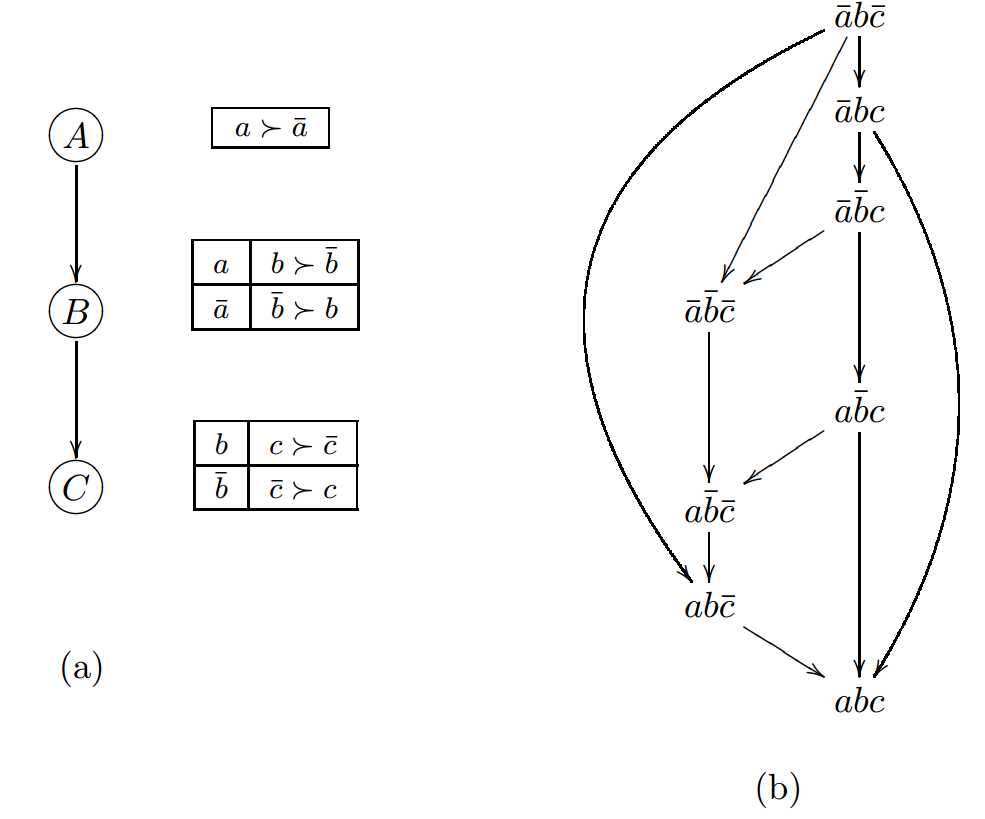
\includegraphics[width=0.7\textwidth]{img/acpn.png}
  \caption{Acyclic CP-net \label{fig:cp_net}}
\end{figure}



\begin{definition}
\label{def:con}
  CP-CONSISTENCY: given a CP-net $N$, decide whether 
	$N$ is consistent.
\end{definition}

Answering the CP-CONSISTENCY problem depends upon whether
its dependency graph are acyclic and how preference rules
in CPTs are specified.
Researchers in AI have been working on this problem
and many results can be found in the literature.
Boutilier, Brafman, Domshlak, Hoos and Poole \cite{bbdh03} 
prove that every acyclic CP-net
is consistent, whereas Goldsmith, Lang, Truszczynski and Wilson \cite{Goldsmith} show
that the CP-CONSISTENCY problem is PSPACE-complete.



\noindent{\textbf{Problems and Complexity.}}
The CP-DOMINANCE problem can be solved by
a polynomial time algorithm for binary-valued tree-structured
CP-nets, and that the problem is NP-complete for binary-valued
CP-nets with specially structured dependency graphs 
(e.g., max-$\delta$-connectedness) \cite{bbdh03}.
However, it is NP-hard for general binary-valued acyclic 
CP-nets \cite{bbdh03}.
Furthermore, in the most general case when the dependency graph
could be cyclic, this problem is proved PSPACE-complete even
if the CP-nets are consistent \cite{Goldsmith}.

The CP-OPTIMALITY-\rom{1} problem is in P, while
the other two optimization problems, namely, the CP-OPTIMALITY-\rom{2}
and CP-OPTIMALITY-\rom{3} problems, seem to have received 
less attention than other problems.



\subsection{Lexicographic Preference Trees \label{sec:LPT}}
\noindent{\textbf{The Language.}}
Let us consider preferences over alternatives from combinatorial domains 
determined by a set $\cI = \{X_1, X_2, \ldots, X_p\}$ of $p$ binary 
\emph{issues}, with each issue
$X_i$ having a binary domain $D(X_i) = \{0_i, 1_i\}$. The 
\emph{combinatorial domain} in question is the set $\cX(\cI)=D(X_1) \times 
D(X_2) \times \ldots\times D(X_p)$. If $\cI$ is implied by the context, 
we write $\cX$ instead of $\cX(\cI)$. For instance, let $\cI = \{X_1, X_2, 
X_3\}$. A 3-tuple $(0_1,1_2,1_3)$ is an alternative from $\cX(\cI)$,
or simply, an alternative over $\cI$. We 
often write it as $0_1 1_2 1_3$ or just as $011$. It assigns $0$ to 
$X_1$, $1$ to $X_2$, and $1$ to $X_3$.  
Clearly, the cardinality of 
$\cX(\cI)$, which we denote by $m$ throughout the paper, is $2^p$. 

A lexicographic preference tree (\emph{LP tree}) $T$ over a set $\cI$ 
of $p$ binary issues $X_1,\ldots,X_p$ is a \emph{binary tree}. Each
node $t$ in $T$ is labeled by an issue from $\cI$, denoted by 
$\mathit{Iss}(t)$, and with \emph{preference information} of the form
$a>b$ or $b>a$ indicating which of the two values $a$ and $b$  comprising
the domain of $\Iss(t)$ is preferred (in general the preference may depend
on the values of issues labeling the ancestor nodes). We require that 
each issue appears exactly once on each path from the root to a leaf. 

Intuitively, the issue labeling the root of an LP tree is of highest 
importance. Alternatives with the preferred value of that issue
are preferred over alternatives with the non-preferred one. The two
subtrees refine that ordering. The left subtree determines the ranking
of the preferred ``upper half'' and the right subtree determines the 
ranking of the non-preferred ``lower half.'' In each case, the same 
principle is used, with the root issue being the most important one. 
\nop{The issue labeling the root of a subtree is the
most important among those appearing in the subtree, and the alternatives
the subtree represents are split into the preferred and non-preferred 
halves based on their value and on the preference information at the node.}
We note that the issues labeling the roots of the 
subtrees need not be the same (the relative importance of issues may 
depend on values for the issues labeling the nodes on the path to the root).

The precise semantics of an LP tree $T$ captures this intuition. Given 
an alternative $x_1x_2\ldots x_p$, we find its preference ranking in 
$T$ by traversing the tree from the root to a leaf. When at node $t$ 
labeled with the issue $X_i$, we follow down to the left subtree if
$x_i$ is preferred according to the preference information at node
$t$. Otherwise, we follow down to the right subtree. 

It is convenient to imagine the existence of yet another level of nodes 
in the tree, not represented explicitly, with each node in the lowest 
explicitly represented level ``splitting'' into two of these
implicit nodes, each representing an alternative. Descending the tree 
given an alternative in the way described above takes us to an (implicit) 
node at the lowest level that represents precisely that alternative.
The more to the left the node representing the alternative, the more 
preferred it is, with the one in the leftmost (implicit) node being the 
most desirable one as left links always correspond to preferred values.

To illustrate these notions, let us consider an example. A group 
of friends in Lexington want to make vacation plans for the 
next year. Having brainstormed for a while, the group decided to focus 
on three binary issues. The \textit{Time} ($X_1$) of the travel could be 
either \textit{summer} ($s$ or $1_1$) or \textit{winter} ($w$ or $0_1$), 
the \textit{Destination} ($X_2$) could be either \textit{Chicago} 
($c$ or $1_2$) or \textit{Miami} ($m$ or $0_2$) and the mode of 
\textit{Transportation} ($X_3$) could be to \textit{drive} ($d$ or $1_3$)
or \textit{fly} ($f$ or $0_3$).
      
Jane, a member of the group, prefers a summer trip to a winter trip, and 
this preference on the issue \textit{Time} is the most important one.  
Then for a summer trip, the next most important issue is \textit{Destination} 
and she prefers Chicago to Miami, and the least important issue is 
\textit{Transportation}. Jane prefers driving to flying if they go
to Chicago, and flying, otherwise.  For a winter trip, the importance of
the remaining two issues changes with \textit{Transportation} being now
more important than the destination -- Jane does not like 
driving in the winter. As for the \textit{Destination}, she prefers to go 
to Miami to avoid the cold weather. These preferences can be captured by 
the LP tree $T$ in Figure \ref{fig:LPTree_full}. We note that the 
trees ordering the vacation plans for summer and for winter are determined 
by trees with different assignments of issues to nodes. For instance, for 
the summer trips, the destination is the most important factor while 
for the winter trips the mode of transportation. The tree shows that
the preferred vacation plan for Jane is to drive to Chicago in 
the summer and the next in order of preference is to fly to Chicago in the 
summer. The least preferred plan is to drive to Chicago in the winter.

\begin{figure}
  \small
	\centering
	\hspace{-1cm}
	\begin{tikzpicture}[->,>=stealth',
	  level/.style={sibling distance=4cm/#1}]
	  \node [main node] (1){Time}
	    child {node [main node] (2) {Dest}
	      child {node [main node] (3) {Tran}}
	      child {node [main node] (4) {Tran}
					child {node [rectangle,draw] at (6.3,4.5) {$s>w$} edge from parent[draw=none]}
					child {node [rectangle,draw] at (0.5,3) {$c>m$} edge from parent[draw=none]}
					child {node [rectangle,draw] at (-0.7,0.6) {$d>f$} edge from parent[draw=none]}
					child {node [rectangle,draw] at (0,0.6) {$f>d$} edge from parent[draw=none]}
					child {node [rectangle,draw] at (2.8,3) {$f>d$} edge from parent[draw=none]}
					child {node [rectangle,draw] at (-0.5,0.6) {$m>c$} edge from parent[draw=none]}
					child {node [rectangle,draw] at (0,0.6) {$m>c$} edge from parent[draw=none]}
				}
	    }
	    child {node [main node] (5) {Tran}
	    child {node [main node] (6) {Dest}}
	      child {node [main node] (7) {Dest}}
	    };
	    \path[every node/.style={font=\sffamily\small}]
	      (1) edge (2)
	          edge (5)
	      (2) edge (3)
	          edge (4)
	      (5) edge (6)
	      		edge (7);
	\end{tikzpicture}
   
  \caption{An LP tree $T$}
  \label{fig:LPTree_full}
\end{figure}

Sometimes LP trees can be represented in a more concise way. For 
instance, if for some node $t$, its two subtrees are identical (that 
is, the corresponding nodes are assigned the same issue), they can be 
collapsed to a single subtree, with the same assignment of issues to 
nodes. To retain preference information, at each node $t'$ of the 
subtree we place a \emph{conditional preference table},
and each preference in it specifies 
the preferred value for the issue labeling that node given the value 
of the issue labeling $t$. In the extreme case when for every node its
two subtrees are identical, the tree can be collapsed to a path. 

Since the preferred issue at a node depends on the values of issues above,
the conditional preference table for the node $t$ located at distance 
$i$ from the root has possibly as many as $2^i$ rows (in general, 
$2^j$ rows, where $j$ is the number of ancestor nodes with one child 
only), with each row specifying a combination of values for the ancestor 
issues together with the preferred value for $\Iss(t)$ given that 
combination. Thus, collapsing subtrees alone does not lead to a smaller 
representation size. However, it can be achieved if there are nodes whose 
preferred value depends only on a limited number of issues labeling 
their single-child ancestor nodes as in such cases the conditional 
preference table can be simplified.  

Formally, given an LP tree (possibly with some subtrees collapsed), for 
a node $t$, let $\ninst(t)$ be the set of ancestor nodes of $t$ whose
subtrees were collapsed into one, and let $\Inst(t)$ represent the 
remaining ancestor nodes. A \emph{parent} function $\cP$ assigns to 
each node $t$ in $T$ a set $\cP(t)\subseteq\ninst(t)$ of \emph{parents}
of $t$, that is, the nodes whose issues may have influence on the local 
preference at $\Iss(t)$. Clearly, the conditional preference table at $t$
requires only $2^{|\cP(t)|}$ rows, possibly many fewer than in the worst 
case. In the extreme case, when an LP tree is a path and each node has 
a bounded (independent of $p$) number of parents, the tree can be 
represented in $O(p)$ space.

If for every node $t$ in an LP tree, $\cP(t)=\emptyset$, all (local)
preferences are unconditional and conditional preference tables consist
of a single entry. Such trees are called \emph{unconditional preference}
LP trees (UP trees, for short). Similarly, LP trees with all non-leaf 
nodes having their subtrees collapsed are called an \emph{unconditional
importance} LP trees (UI trees, for short). This leads to a a natural 
classification of LP trees into four classes: unconditional importance 
and unconditional preference LP trees (UI-IP trees), unconditional 
importance and conditional preference trees (UI-CP trees), etc. The class
of CI-CP trees comprises all LP trees, the class of UI-UP trees is the 
most narrow one. 

The LP tree $T$ in Figure \ref{fig:LPTree_full} can be represented more
concisely as a (collapsed) CI-CP tree $v$ in Figure \ref{fig:LPTree}. Nodes
at depth one have their subtrees collapsed. In the tree in Figure
\ref{fig:LPTree_full}, the subtrees of the node at depth 1 labeled 
\textit{Tran} are not only identical but also have the same preference 
information at every node. Thus, collapsing them does not incur growth in
the size of the conditional preference table.
      
\begin{figure}
   \small
	\centering

  \begin{tikzpicture}[->,>=stealth',node distance=2cm,main node/.style={circle,draw,font=\small}]
        
    \node[main node] (1) {Time};
    \node[rectangle,draw] at (1.2,0) {$s > w$};
    
    \node[main node] (2) [below left of=1] {Dest};
    \node[rectangle,draw] at (-2.6,-1.4) {$c > m$};
		%\node[rectangle] at (-2.0,-1.4) {$t'$};
    
    \node[main node] (3) [below of=2] {Tran};
    \node[rectangle split, rectangle split parts=2, draw, font=\sffamily\small] at (-2.9,-3.5)
        {
          $c:d>f$
          \nodepart{second}
          $m:f>d$
        };
    %\node[rectangle] at (-2,-3.5) {$t$};
    
    \node[main node] (4) [below right of=1] {Tran};
    \node[rectangle,draw] at (2.6,-1.4) {$f > d$};
    
    \node[main node] (5) [below of=4] {Dest};
    \node[rectangle,draw] at (2.6,-3.4) {$m > c$};
  
    \path[every node/.style={font=\sffamily\small}]
      (1) edge (2)
          edge (4)
      (2) edge (3)
      (4) edge (5);
  \end{tikzpicture}
  
%  \vspace{-0.3cm}
  \caption{An CI-CP LP tree $T$}
  \label{fig:LPTree}
%  \vspace{-0.5cm}
\end{figure}

\noindent{\textbf{The Model.}}
An LP tree consisting of $p$ binary issues corresponds to a strict total order over
$2^p$ alternatives.  For the example in \figref{LPTree}, the total order induced
by $T$ is
\begin{center}
	$scd \succ scf \succ smf \succ smd \succ wmf \succ wcf \succ wmd \succ wcd$.
\end{center}

\noindent{\textbf{Problems and Complexity.}}
An LP tree orders pairs of alternatives ($M,M'$) by traversing down the tree
and check the issues accordingly until an issue $X$ is reach such that
$M(X) \not = M'(X)$.  $M$ and $M'$ are then ordered based on the preference
information on $X$ \cite{booth:learningLP}.  Thus, we have the following 
\thmref{LP_DOM}.

\begin{thm}
\label{thm:LP_DOM}
	The $\LP$-DOMINANCE problem can be solved in time linear in $p$.
\end{thm}
\begin{proof}
	The linear time algorithm is shown in \algref{LP_dom}.

	\begin{algorithm}[ht]
	\KwIn{an LP tree $T$, two alternatives $M$ and $M'$ ($M \not = M'$)}
	\KwOut{$\true$ if $M' \succ_T M$; $\false$, otherwise}
	Let $T^* = T$\;
	\For{$i \leftarrow 1$ \KwTo $p$}{
	  Let $X_j$ be the root of $T^*$ with preference $x_j \succ \bar{x_j}$\;
	  
	  \uIf{$M'(X_j) > M(X_j)$}{
			\Return{$\true$}\;
	  }
		\uElseIf{$M'(X_j) < M(X_j)$}
		{
			\Return{$\false$}\;
	  }
		\Else{
			$T^* \leftarrow T^*(x_j)$\;
		}
	}
	
	\caption{Solving the $\LP$-DOMINANCE problem\label{alg:LP_dom}}
	\end{algorithm}
\end{proof}

Since an LP tree determines a linear order over alternatives, an optimal
alternative always exists and the $\LP$-OPTIMALITY-\rom{1} problem
is trivial.  And it can be solved in time linear in $p$.
Similarly, the $\LP$-OPTIMALITY-\rom{2} and
$\LP$-OPTIMALITY-\rom{3} problems are easy to solve.

Instead of the problems of reasoning about a single
LP tree, recently researchers have studied
the problem of aggregating LP trees from multiple
agents to facilitate collaborative decision making.
LP trees are aggregated
according to some social choice scheme, such as
issue-by-issue voting \cite{fargier:ibi},
sequential majority voting rule \cite{Xia:SMV},
positional scoring rules (e.g. Borda, $k$-Approval) \cite{lang,LiuT}.
In \chref{aggLP}, I will provide detailed definitions of aggregating
problems and results I obtained on their complexity 
according to positional scoring rules, as
well as experimental analysis for two computational tools:
Answer Set Programming (ASP) \cite{aspataglance} and 
Weighted Partial Maximum Satisfiability (WPM) \cite{papado:b:compcomplexity}.

\subsection{Conditional Preference Theories}
The formalism of conditional preference theories was proposed by
Wilson \cite{Wilson04extendingcp-nets}.
Conditional Preference Theories (\textit{CP theories}) allows
compact representation of certain kinds of conditional preference
statements.
The logic generalizes both CP-net \cite{Wilson04extendingcp-nets} and TCP-net
\cite{WilsonECAI04}.

\noindent{\textbf{The Language.}}
In the language of CP-nets, one can express her preferences over cars
under the semantics of \textit{ceteris paribus} as follows:
\textit{A Toyota car is preferred to a Ford car, everything else being equal}.
Such semantics of CP-nets imposes limitation on its expressivity for
stronger preference statements, such as
\textit{A Toyota car is preferred to a Ford car, regardless of how they
evaluate the other variables}.
CP-nets cannot generally express such statements in a compact way
\cite{Wilson04extendingcp-nets}, while CP theories can.

\begin{definition}
	Let $V$ be a set of variables.  For each $X\in V$, let $\underline{X}$
	be the set of values of $X$.  For each $U \subset V$, let
	$\underline{U}=\Pi_{X\in U} \underline{X}$ be the set of assignments to $U$.
	A conditional preference statement $\varphi$ is of the form
	\begin{center}
		$u : x > x' [W]$,
	\end{center}
	where $u \in \underline{U}$, $x,x' \in \underline{X}$ ($X \not \in U$),
	and $W \subseteq V-U-\{W\}$.
	A conditional preference theory $\Gamma$ is a set of 
	conditional preference statements.
\end{definition}

\nop{\mc{
	Need an example of CPTh here.
}}

\noindent{\textbf{The Model.}}
\begin{definition}
	For $\varphi=u:x>x'[W]$, let $T \subseteq V$ be
	$V-\{U \cup \{X\} \cup W\}$.
	Define $\varphi^*$ the set of pairs of outcomes
	$\{(tuxw,tux'w'):t\in \underline{T}, w,w' \in \underline{W}\}$ induced
	by $\varphi$.
\end{definition}
Each pair $(\alpha,\beta) \in \varphi^*$ represents the preference of
$\alpha$ over $\beta$.  Informally, $\varphi$ expresses that,
given $u$, $x$ is preferred to $x'$ regardless of the assignments $w,w'$
to $W$, everything else (assignments $t$ to $T$) being equal.
Consider a set of cars over three binary variables \textit{Make}, \textit{Color}
and \textit{Category}, where $\Dom(Make)=\{Toyota(t),Ford(f)\}$,
$\Dom(Color)=\{black(b),white(w)\}$, and $\Dom(Category)=\{sedan(s), truck(r)\}$.
For a preference over cars
``\textit{For Toyota cars, a sedan is preferred to a truck, regardless of other variables},"
we have the following preference statement $\varphi$:
\begin{center}
	$\textit{Toyota} : \textit{sedan} > \textit{truck} \, [\{Color\}]$.
\end{center}
We see that $\varphi$ is a shorthand for the set $\varphi^*$ of four binary relations
it induces:
$tbs \succ tbr$, $tbs \succ twr$, $tws \succ tbr$, and $tws \succ twr$.


\begin{definition}
	Let $\Gamma$ be a conditional preference theory, define $\Gamma^*$
	the union of $\varphi^*$ for all $\varphi$ in $\Gamma$, that is,
	$\Gamma^* = \bigcup_{\varphi \in \Gamma} \varphi^*$.
	Assume preference relation is transitive, define $>_{\Gamma}$
	the transitive closure of $\Gamma^*$.
\end{definition}

We define models of $\Gamma$ to be strict total orders on $\underline{V}$.
\begin{definition}
	Let $>$ be a strict total order on $\underline{V}$.
	The relation $>$ is a model of $\phi$, $> \models \varphi$ if and only if
	$> \supseteq \phi^*$.  
	The relation $>$ is a model of $\Gamma$, $> \models \Gamma$, if and only if 
	$> \supseteq \Gamma^*$.
	We say $\Gamma$ is consistent if it has a model, that is, 
	there exists a strict total order $>$
	such that $> \models \Gamma$.
\end{definition}

Indeed, we have $> \models \varphi$ if and only if $\alpha > \beta$ whenever
$(\alpha,\beta) \in \varphi^*$.  That is, for all $t \in \underline{T}$ and
$w,w' \in \underline{W}$, $tuxw > tux'w'$.


\noindent{\textbf{Problems and Complexity.}}
Let $\Gamma$ be a CP theory, $G(\Gamma)$ a directed graph with edges
representing dependency and importance relations.
Assuming $G(\Gamma)$ is acyclic,
sufficient and necessary conditions for a CP theory to be consistent
have been characterized \cite{Wilson04extendingcp-nets}:
The CP theory $\Gamma$ is consistent if and only if
$\Gamma$ is locally consistent.
Under this assumption, the CPTh-CONSISTENCY problem can be solved
efficiently.  Moreover, computing a model of $\Gamma$ and 
finding an optimal outcome can also be solved in polynomial time
by constructing from $\Gamma$ a partial conditional lexicographic order
which can easily be extended to a total order
\cite{Wilson04extendingcp-nets}.
Other sufficient conditions of consistency are discussed too
\cite{WilsonECAI04}.

In general, the CPTh-DOMINANCE problem is PSPACE-complete
\cite{Wilson:2006:EUA:1567016.1567119}.


\subsection{Answer Set Optimization}
The formalism of Answer Set Optimization (ASO) was originally introduced by
Brewka, Nieml\"a and Truszczynski \cite{Brewka03answerset} and
later enhanced by Brewka \cite{Brewka04}.
%A declarative planning language, $\cPP$, was introduced \cite{Son:plan_pref}
%and shown that any preference in $\cPP$ can be embedded in ASO preferences
%\cite{Brewka04}.

In this work, we focus on the original framework \cite{Brewka03answerset} where 
the Pareto method is used to order outcomes.
Other methods can be found in the latter paper \cite{Brewka04}.
In more recent works \cite{Faber:QOP,Faber:APF}, 
the Pareto-based ASO framework is generalized in the setting of
qualitative optimization problems.


\noindent{\textbf{The Language.}}
\begin{definition}
	Let $A$ be a finite set of atoms.
	An ASO theory over $A$ is a tuple $(P_{\gen},P_{\PREF})$, where
	\begin{enumerate} \itemsep -4pt
		\item $P_{\gen}$, the generating program, is a logic program
					with hard constraints, built of atoms in $A$,
					used to generate answer sets called feasible outcomes,
		\item $P_{\PREF}$, the selecting program, is a preference
					program consisting of preference rules of the form
			\begin{center}
				$\gamma_1 > \ldots > \gamma_k \leftarrow \alpha$,
			\end{center}
					where each $\gamma_i$ is a propositional formula
					over $A$ and $\alpha$ is a conjunction of
					literals of atoms in $A$.
	\end{enumerate}
\end{definition}

\nop{\mc{
	Need to show an example of ASO here.
}}

\noindent{\textbf{The Model.}} 
A single ASO preference rule specifies a total preorder over outcomes, while,
applying the Pareto ordering, a general ASO program with multiple preferences
describe a partial preorder over the space of answer sets.

We say outcome $o$ is \tit{irrelevant} to preference rule $r$ if
$o \models (\neg \alpha) \vee (\neg \gamma_1 \wedge \ldots \wedge \gamma_k)$,
that is, $o$ does not satisfy $\alpha$ or $o$ does not satisfy any of
the Boolean combinations. As mentioned in the work by Brewka et al \cite{Brewka03answerset},
outcomes irrelevant to $r$ are considered as good as the
best outcomes.
This default treatment of irrelevance can be overwritten by
including formula $(\neg \alpha) \vee (\neg \gamma_1 \wedge \ldots \wedge \gamma_k)$
in any place of the preference rule $r$.
Formally we define satisfaction degree of an answer set with respect to a
preference rule.
\begin{definition}
	Let $o$ be an outcome generated by $P_{\gen}$,
	$r$ an ASO preference rule.
	The satisfaction degree of $o$ on $r$, denoted $d_r(0)$,
	is defined as follows: $d_r(o)=1$ if $o$ is irrelevant to $r$;
	$d_r(o)=\min\{i:o \models \gamma_i\}$, otherwise.
\end{definition}

\begin{definition}
	Let $(P_{\gen}, P_{\PREF})$ be an ASO theory,
	$o$ and $o'$ two outcomes.
	$o'$ is weakly Pareto-preferred to $o$, $o' \succeq o$,
	if $\forall r \in P_{\PREF}, d_r(o') \leq d_r(o)$.
	$o'$ is strictly Pareto-preferred to $o$, $o' \succ o$,
	if $o' \succeq o$ and $o \not \succeq o'$.
	$o$ is optimal if there exists no outcome $o''$ such that
	$o'' \succ o$.
\end{definition}

Consider an ASO theory $P=(P_{\gen}, P_{\PREF})$, where
\begin{center}
	$P_{\gen}=\{$
	$(a \lor \bar{a}) \land (\neg (a \land \bar{a})). \;$
	$(b \lor \bar{b}) \land (\neg (b \land \bar{b})). \;$
	$(c \lor \bar{c}) \land (\neg (c \land \bar{c})). \;$
	and\\
	$P_{\PREF}=\{
		a > \bar{a} \leftarrow b \vee c. \;\;
		b \wedge \bar{c} > \bar{b} \wedge c.
	\}$.
\end{center}
An optimal outcome is $ab\bar{c}$ and it is the only optimal one.

\noindent{\textbf{Problems and Complexity.}}
Brewka et al \cite{Brewka03answerset} proved that
the ASO-DOMINANCE problem is in P, ASO-OPTIMALITY-\rom{1}
is NP-complete, ASO-OPTIMALITY-\rom{2} is coNP-complete,
and ASO-OPTIMALITY-\rom{3} is $\sigmap{2}$-complete.

Moreover, an extended paradigm of ranked ASO programs has
been introduced in the same work \cite{Brewka03answerset}.
Ranked ASO programs are ASO programs where rules in $P_{\PREF}$
are given numeric values that represent different levels of importance
of preference rules.  Nonetheless, complexity results presented
above stay unchanged.




\section{Social Choice}
The study of preference aggregation can be traced back to social choice theory,
which dates back to Condorcet's paradox of voting, noted by the
Marquis de Condorcet in the 18th century, in which
the winning ranking of alternatives could be cyclic even 
given acyclic individual votes \cite{wiki:soc}.
Kenneth Arrow's work, \textit{Social Choice and Individual Values},
is recognized as the basis of modern social choice \cite{aarrow:b:socialchoice}.
In the book, Arrow states that any preference aggregation method for at least three
alternatives cannot meet some fairly desirable axioms, a result known as
the Arrow's impossibility theorem.
Extending this result, Gibbard and Satterthwaite showed
that any social choice function, again meeting some fair properties, is subject
to manipulation \cite{gib:j:maip-scheme,satt:j:strat-proof}.
Extending the Gibbard-Satterthwaite theorem, the Duggan-Schwartz theorem deals with 
voting rules that elect a nonempty set of co-winners rather than a single winner
\cite{dug-sch:j:maipres}.

All these results inform us that it is impossible to design a fair preference
aggregation system that is manipulation-proof.
However, Bartholdi, Tovey and Trick proposed the idea of protecting
social choice schemes from manipulation via computational
complexity \cite{bartholdi:j:whowon,bartholdi:j:compdiff,
bartholdi:j:howhard}.
The idea is that, if manipulation is computationally hard to
achieve, manipulation is unlikely.

That started the field of computational social choice by adding an algorithmic
perspective from computer science to the formal approach 
of social choice theory \cite{Brandt:COMSOC}.




\subsection{Preference Aggregation}
One of the most fundamental problems in social choice theory is how to
aggregate individual preferences over alternatives so that a
collaborative preference relation is reached.
In other settings, people are interested in some optimal alternatives
rather than a collective preference relation over all alternatives.

\noindent{\textbf{Social Welfare Functions.}}
\begin{definition}
	Let $A=\{a_1,\ldots,a_m\}$ be a finite set of alternatives,
	$N=\{1,\ldots,n\}$ a finite set of agents (or voters).
	A preference relation (or a vote) $v_i$ given by agent $i$ 
	is a strict total order $\succ_i$,
	that is, a total, transitive and antisymmetric.
	A preference profile $P$ is a finite set of preference relations
	$\{\succ_1, \ldots, \succ_n\}$.
\end{definition}

We denote by $\cL(A)$ the set of all preference relations over
the space of alternatives $A$, and $\cL(A)^n$, the set of all
preference profiles.

\begin{definition}
	A social welfare function ($\SWF$) is a function $f$:
	\begin{center}
		$\cL(A)^n \rightarrow \cL(A)$.
	\end{center}
	We call the resulting relation $\succ$ the social preference relation.
\end{definition}

If there are two alternatives $a_1$ and $a_2$,
May's theorem \cite{May52} suggests that $a_1$ should be
preferred to $a_2$ in the social preference relation
if and only if more agents prefer $a_1$ to $a_2$ than
$a_2$ to $a_1$.
This idea is called the majority voting.
However, when there are more than two alternatives,
the majority voting rule can lead to cycles of
alternatives, which is known as the Condorcet's paradox.
For instance, we have three voters with the following
preference relations:
\begin{center}
	$a_1 \succ_1 a_2 \succ_1 a_3$\\
	$a_2 \succ_2 a_3 \succ_2 a_1$\\
	$a_3 \succ_3 a_1 \succ_3 a_2$
\end{center}
Based on the pairwise majority rule, we have the following cycle
\begin{center}
	$a_1 \succ a_2$, $a_2 \succ a_3$, $a_3 \succ a_1$. 
\end{center}

A general result, Arrow's theorem, shows that no social welfare
functions satisfies some fairness conditions, defined as follows.

\begin{definition}
	An $\SWF$ satisfies \textit{Pareto efficiency} if 
	\begin{center}
		$\forall i \in N, \forall a_j,a_k \in A, (a_j \succ_i a_k \Rightarrow a_j \succ a_k)$.
	\end{center}
	Let $N_{(a_j,a_k)}$ be the set of voters where
	$a_j$ is preferred to $a_k$ ($N_{(a_j,a_k)}=\{i:a_j \succ_i a_k\}$).
	An $\SWF$ satisfies \textit{independence of irrelevant alternatives} if
	\begin{center}
		$\forall P,P' \in \cL(A)^n, \forall a_j,a_k \in A, (N_{(a_j,a_k)}=N'_{(a_j,a_k)}\Rightarrow$\\
		$a_j,a_k$ are ranked identically in $\succ$ and $\succ')$.
	\end{center}
	An $\SWF$ satisfies \textit{non-dictatorship} if there is no agent $i$ such that
	\begin{center}
		$\forall P \in \cL(A)^n, \forall a_j,a_k \in A, (a_j \succ_i a_k \rightarrow a_j \succ a_k)$.
	\end{center}
\end{definition}

\begin{thm}
\label{thm:Arrow}
\emph{(Arrow, 1951)}
	When there are at least three alternatives,
	There exists no $\SWF$ that simultaneously satisfies
	Pareto efficiency, independence of irrelevant alternatives
	and non-dictatorship.
\end{thm}



\noindent{\textbf{Social Choice Functions.}}
\begin{definition}
	A social choice function ($\SCF$) is a function $f$:
	\begin{center}
		$\cL(A)^n \rightarrow 2^A-\{\emptyset\}$.
	\end{center}
	We call the resulting alternative (alternatives)
	a winner (co-winners, respectively).
\end{definition}

We now discuss some of the desirable axioms of an $\SCF$ including
resolution, anonymity and neutrality.
Note that the axioms for $\SWF$ may not directly apply here.

\begin{definition}
	An $\SCF$ $f$ is resolute if it always yields a unique winning alternative, that is,
	\begin{center}
		$\forall P \in \cL(A)^n, |f(P)|=1$.
	\end{center}
	$f$ is anonymous if names of the voters do not matter, that is,
	for every permutation $\pi$ on voters,
	\begin{center}
		$f({v_1,\ldots,v_n}) = f(v_{\pi(1)},\ldots,v_{\pi(n)})$.
	\end{center}
	$f$ is neutral if names of the alternatives do not matter, that is,
	for every profile $P$ and every permutation $\pi$ on alternatives,
	\begin{center}
		$\pi(f(P)) = f(\pi(P))$.
	\end{center}
\end{definition}

Surprisingly, these three fairness conditions cannot be satisfied simultaneously
by any $\SCF$. We have the following easy impossibility theorem \cite{Brandt:COMSOC}.

\begin{thm}
\label{thm:easy}
	A resolute $\SCF$ cannot satisfy both anonymity and neutrality.
\end{thm}
%\begin{proof}
%	Consider the election with two votes over two alternatives $a$ and $b$:
%	\begin{center}
%		$P=\{a \succ_1 b, b \succ_2 a\}$.
%	\end{center}
%	We apply the resolute $\SCF$: the majority rule with tie-breaking in favor of $a$.
%	So $a$ wins in $P$.
%	Assuming anonymity, we still have $a$ as the winner in profile $P'$:
%	\begin{center}
%		$P'=\{a \succ_2 b,b \succ_1 a\}$.
%	\end{center}
%	Let us assume neutrality also holds, $b$ wins in $P'$.  Contradiction!
%
%\end{proof}

%The three axioms discussed in Arrow's theorem need adjusting 
%in the setting of social choice functions.
%Below we show how Pareto efficiency and non-dictatorship are aligned.
%
%\begin{definition}
%	An $\SCF$ $f$ satisfies \textit{Pareto efficiency} if 
%	\begin{center}
%		$\forall v_i \in P, \forall a_j,a_k \in A, (a_j \succ_i a_k \Rightarrow a_k \not \in f(P))$.
%	\end{center}
%	An $\SCF$ satisfies \textit{non-dictatorship} if there is no agent $i$ such that
%	\begin{center}
%		$\forall P \in \cL(A)^n, (a=\topFunc(v_i) \Rightarrow a \in f(P))$,
%	\end{center}
%	where $\topFunc(v_i)$ returns the top ranked alternative in vote $v_i$.
%\end{definition}
%
%\begin{definition}
%	An $\SCF$ $f$ satisfies \textit{liberalism} if 
%	for every agent $i \in N$, there are two different alternatives $a,b \in A$ such that
%	\begin{center}
%		$i \in P_{(a,b)} \Rightarrow b \not \in f(P)$ and $i \in P_{(b,a)} \Rightarrow a \not \in f(P)$.
%	\end{center}
%\end{definition}
%
%The following theorem by A. Sen \cite{Sen} states the impossibility of an $\SCF$ satisfying
%both Pareto efficiency and liberalism.
%
%\begin{thm}
%\label{thm:Sen}
%\emph{(Sen, 1971)}
%	When there are at least two agents,
%	there exists no $\SCF$ that simultaneously satisfies
%	Pareto efficiency and liberalism.
%\end{thm}

Another desirable property of an $\SCF$ is that if the support of a winning
alternative grows then it stays a winner in the new profile.
This condition is called monotonicity. Formally, we define monotonicity as follows.

\begin{definition}
	An $\SCF$ $f$ satisfies \textit{monotonicity} if 
	\begin{center}
		$\forall a,b \in A, \forall P,P' \in \cL(A)^n, (a \in f(P) \wedge 
		N_{(a,b)} \subseteq N'_{(a,b)} \Rightarrow a \in f(P'))$.
	\end{center}
\end{definition}

For instance, the majority rule (plurality) does not satisfy monotonicity, but 
the Condorcet rule does.  Another desired property is that every alternative
has a chance to win, namely, surjectivity (or non-imposingness).  More formally, 
an $\SCF$ $f$ is surjective if for every alternative $a \in A$, there exists
some profile $P$ such that $a \in f(P)$.
Regarding the aforementioned two fairness conditions, Muller and Satterthwaite \cite{Mull_Satt}
proved yet another impossibility theorem for $\SCF$'s.

\begin{thm}
\label{thm:Mull_Satt}
\emph{(Muller and Satterthwaite, 1977)}
	When there are at least three alternatives,
	any resolute $\SCF$ satisfying monotonicity and surjectivity is dictatorial.
\end{thm}



\subsection{Voting Rules}
We first define voting rules.

\begin{definition}
	A voting rule $r$ is a specific $\SCF$ proposed for practical use.
\end{definition}

\noindent{\textbf{Positional Scoring Rules.}}
For profiles over a set $A$ of alternatives, 
a \emph{scoring vector} is a sequence $w= (w_1,\ldots,
w_m)$ of integers such that $w_1\geq w_2 \geq \ldots \geq w_m$
and $w_1 > w_m$. Given a vote
$v$ with the alternative $a$ in position $i$ ($1 \leq i \leq m$), 
the score of $a$ in
$v$ is given
by $s_w(v,a)=w_i$. Given a profile $P$ of votes and an alternative $a$,
the score of $a$ in $P$ is given by $s_w(P,a) = \sum_{v\in P} s_w(v,a)$. 
These scores determine the ranking generated from $P$ by the scoring
vector $w$ (assuming, as is common, some independent tie breaking rule). 
Common positional scoring rules include the plurality rule,
the veto rule, the $k$-approval rule and Borda's rule.
\begin{enumerate} \itemsep -4pt
	\item plurality: $(1,0,\ldots,0)$
	\item veto: $(1,\ldots,1,0)$
	\item $k$-approval: $(1,\ldots 1,0,\ldots 0)$ with $k$ the number of 1's
	\item Borda: $(m-1,m-2,\ldots, 1,0)$
\end{enumerate}

We propose yet another positional scoring rule, called $(k,l)$-approval \cite{LiuT},
with the scoring vector $(a,\ldots,a,b,\ldots,b,0,\ldots,0)$, where
both $a$ and $b$ are constants $(a \geq b)$ and the numbers of $a$'s and $b$'s equal to
$k$ and $l$, respectively.
Note that $(k,l)$-approval allows agents to specify two levels of approval,
compared to only one level in $k$-approval, and thus $(k,l)$-approval
generalizes $k$-approval.

A voting method, that is closely related to positional scoring rules, is
the approval voting \cite{BraFis}.
Under approval voting, each voter approves any number of alternatives
and the winner, or co-winners, are those with the highest score.

\noindent{\textbf{Condorcet Consistent Rules.}}
A \tit{Condorcet winner} is an alternative that wins every pairwise comparisons
against each of the other alternatives.
Clearly, a Condorcet winner is unique whenever it exists.
If a voting rule $r$ always selects the Condorcet winner,
if it exists, then $r$ is said to be Condorcet consistent.

Positional scoring rules are not Condorcet consistent \cite{Fis}.
Voting rules that are Condorcet consistent include the following,
only to list a few \cite{Brandt:COMSOC}.
\begin{enumerate} \itemsep -4pt
	\item Copeland's rule: An alternative scores 1 for each pairwise comparison
				it wins, and some number between 0 and 1 for each pairwise comparison
				it ties.  Alternatives with the highest score are the co-winners.
	\item Maximin: The Maximin score of an alternative $a$ is the minimum number of
				votes for $a$ among all pairwise comparisons.  
				Alternatives with the highest Maximin score wins.
	\item Kemeny's rule: It selects linear rankings that maximize the number of agreements 
				with pairwise preferences of alternatives in the profile of votes, and
				the top-ranked alternatives in these rankings are the co-winners.
	\item Dodgson's rule: A winner is an alternative that can be made a Condorcet winner 
				by a minimal number of swaps of adjacent alternatives in the votes.
\end{enumerate}

If it is required that only a single winner is eventually elected,
we apply some tie-breaking method in case of co-winners.
Such a tie-breaking method could be that we break ties in favor of
the lexicographically smallest or largest alternative, or in favor of
a randomly picked alternative among co-winners.



%\noindent{\textbf{Other Rules.}}




\subsection{Manipulation \label{sec:manip}}
In practice, preference relations, or votes, are collected from voters
who could report preferences that are not truthful.
The reason why any agent would do so is that
casting an untruthful vote, under certain circumstances,
may benefit the agent in that she could end up with
a better result, compared to the result of the election
with her true preferences.
In cases when an agent can be better off misreporting her
true preferences, we say that she can perform manipulation.
Assuming a voting rule is resolute,
we define manipulability as follows.

\begin{definition}
	A resolute voting rule $f$ is manipulable if there exist
	a voter $i \in N$ and preference profiles $P,P' \in \cL(A)^n$
	such that $P-v_i=P'-v_i'$ and $f(P) \succ_i f(P')$.
	A voting rule is strategy-proof if not manipulable.
\end{definition}

Since manipulation seems undesirable, researchers are
interested in determining what voting rules are
manipulable and what are not.
Surprisingly, as shown in the Gibbard-Satterthwaite
theorem \cite{gib:j:maip-scheme,satt:j:strat-proof},
any reasonable voting rule is susceptible to
manipulation given that the number of alternatives
is at least three.

\begin{thm}
\label{thm:Gib_Sat}
\emph{(Gibbard, 1973; Satterthwaite, 1975).}
	When there are at least three alternatives,
	every resolute, surjective, strategy-proof voting rule is
	dictatorial.
\end{thm}

Since it is impossible to have any reasonable voting rule that is strategy-proof,
researchers have worked hard to circumvent the theorem
for strategy-proof voting rules by restricting the domains
of preferences\cite{Brandt:COMSOC}.
Moulin \cite{Moul} observed that any voting rule uniquely selecting
the Condorcet winner is strategy-proof, assuming the existence
of Condorcet winners in any profile of preference relations
expressed in a restricted domain.
One such domain is the domain of single-peaked preferences
\cite{Sprumont}.

\noindent{\textbf{Computational Hardness of Manipulation.}}
In spite of the fact that voting rules can be strategy-proof
when preferences are restricted, in practice we cannot impose
constraints onto how agents should formulate their preferences.
Another approach to work around the impossibility theorem is
to protect voting rules against manipulation by showing
high computational complexity.

We first give a definition of the manipulation problem as follows.
\begin{definition}
	Let $r$ be a resolute voting rule.  Given a profile $P$ of
	$n$ votes over $m$ alternatives and an alternative $c$, 
	the manipulation problem is to decide whether there exists
	a single vote $v'$ such that $c=r(P \cup \{v'\})$.
\end{definition}

The manipulation problem is proved to be NP-hard for several
rules, such as second-order Copeland (SOC) \cite{bartholdi:j:compdiff}, and
single transferable vote (STV) \cite{Bartholdi:STV}.
A variant of the manipulation problem is
called coalitional manipulation problem, where 
manipulative voters jointly make $c$ a winner.
Since the manipulation problem defined above is
a special case of this variant, both SOC and STV
are NP-hard.  Additionally, the variant is
also NP-hard for Copeland \cite{Faliszewski:Copeland},
maximin \cite{xia2009complexity} and Borda 
\cite{betzler2011unweighted,davies2011complexity}.

